% !TEX root = ../main.tex

\section{New mitigations}

By this point, we have discussed 10 solutions to the multiple withdrawal attack and we evaluated them in terms of compatibility with the standard and attack mitigation (recall the summary in Table~\ref{tab:comp}). Since none of them precisely satisfy the constraints of the ERC20 standard, we now propose two new solutions to mitigate the attack.

\subsection{Proposal 1: Securing \textit{approve} method}

As discussed in the previous section, a sustainable solution should use CAS pattern\cite{Ref06} to set new allowance atomically. This needs knowledge of transferred tokens that requires adding a new mapping variable to the token code. The code is still compatible with other smart contracts due to internal usage of the variable. Modified version of \textit{transferFrom} method can track transferred tokens by storing them in this new variable (\textit{transferred}):

\begin{figure}[t]
	\centering
	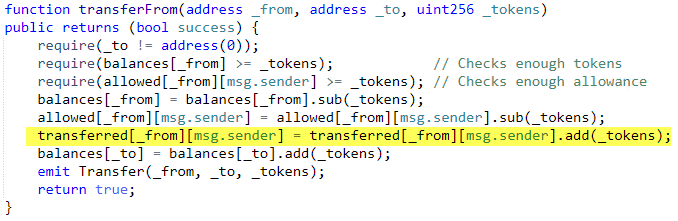
\includegraphics[width=1.0\linewidth]{figures/multiple_withdrawal_14.png}
	\caption{Modified version of \textit{transferFrom} for keeping track of transferred tokens per spender.}
\end{figure}

Similarly, a block of code is added to the \textit{approve} function to work in both cases with zero and non-zero allowances. Added code compares new allowance (passed as \textit{\_tokens} to the function) with the current allowance of the spender and already transferred token (highlighted as \textit{allowed[msg.sender][\_spender]} and \textit{transferred[msg.sender][\_spender]} respectively). Then it decides to increase or decrease current allowance based on this comparison. If the new allowance is less than initial allowance (sum of \textit{allowance} and \textit{transferred} variables), it denotes decreasing allowance, otherwise increasing allowance was intended.

\begin{figure}[t]
	\centering
	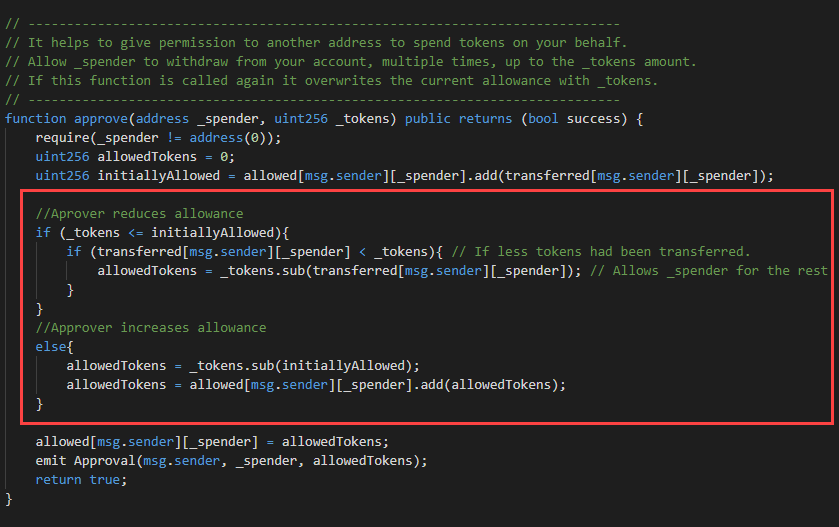
\includegraphics[width=1.0\linewidth]{figures/multiple_withdrawal_15.png}
	\caption{Added code block to \textit{approve} function to prevent the attack by comparing and setting new allowance atomically.}
\end{figure}

Modified \textit{approve} function prevents the attack in either increasing or decreasing of the allowance. Unlike other solutions, there is no need to set allowance from N to 0 and then to M. The owner can directly change the allowance from N to M which is saving one transaction accordingly. Considering the below scenarios when decreasing or increasing allowance.

\subsubsection*{Scenario A} Alice approves Bob for spending 100 tokens and then decides to decrease it to 10 tokens.
\begin{enumerate}
	\item Alice approves Bob for transferring 100 tokens.
	\item After a while, Alice decides to reduce Bob’s allowance from 100 to 10 tokens.
	\item Bob noticed Alice’s new transaction and transfers 100 tokens by front-running.
	\item Bob’s allowance is 0 and \textit{transferred} is 100 (set by \textit{transferFrom} function).
	\item Alice’s transaction is mined and checks initial allowance (100) with new allowance (10).
	\item As it is reducing, \textit{transferred} tokens (100) is compared with new allowance (10). Since Bob already transferred more tokens, his allowance will be set to 0.
	\item Bob is not able to move more than initial 100 approved tokens.\newline
\end{enumerate}

\subsubsection*{Scenario B} Alice approves Bob for spending 100 tokens and then decides to increase it to 120 tokens.
\begin{enumerate}
	\item Alice approves Bob for transferring 100 tokens.
	\item After a while, Alice decides to increase Bob’s allowance from 100 to 120 tokens.
	\item Bob noticed Alice’s new transaction and transfers 100 tokens by front-running.
	\item Bob’s allowance is 0 and \textit{transferred} is 100.
	\item Alice’s transaction is mined and checks initial allowance (100) with new allowance (120).
	\item As it is increasing, new allowance (120) will be subtracted from transferred tokens (100).
	\item 20 tokens will be added to Bob’s allowance.
	\item Bob would be able to transfer more 20 tokens (120 in total as Alice wanted).\newline
\end{enumerate}

In order to evaluate functionality of the new \textit{approve}/\textit{transferFrom} functions, we have implemented a standard ERC20 token (TKNv1\footnote{https://rinkeby.etherscan.io/address/0x8825bac68a3f6939c296a40fc8078\newline d18c2f66ac7}) along side proposed ERC20 token (TKNv2\footnote{https://rinkeby.etherscan.io/address/0xf2b34125223ee54dff48f71567d4b\newline 2a4a0c9858b}) on Rinkeby test network. Result of tests for different input values shows that TKNv2 can address multiple withdrawal attack by making front-running gain ineffective. Moreover, we compared these two tokens in term of gas consumption. TokenV2.\textit{approve} function uses almost the same amount of gas as TokenV1.\textit{approve}, however, gas consumption of TokenV2.\textit{transferFrom} is around 47\% more than TokenV1.\textit{transferFrom}. This difference is because of maintaining a new mapping variable for tracking transferred tokens:

\begin{figure}[t]
	\centering
	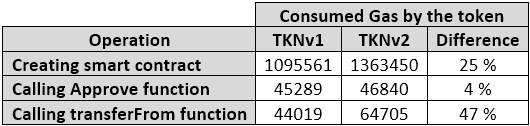
\includegraphics[width=1.0\linewidth]{figures/multiple_withdrawal_22.png}
	\caption{Comparison of gas consumption between standard implementation of ERC20 token (TKNv1) and secured implemetation (TKNv2).}
\end{figure}

In term of compatibly, working with standard wallets (like MetaMask) have not raised any transfer issue. This shows compatibility of the token with existing wallets. In summary, we could use CAS pattern to implement a secure \textit{approve} method that can mitigate the attack effectively. However, it violates one of ERC20 specifications that says "If this function is called again it overwrites the current allowance with \textit{\_value}". This implementation of \textit{approve} method adjusts allowance based on transferred tokens. Essentially, it would not be possible to secure the \textit{approve} method without adjusting the allowance. Considering the below scenario:

\begin{enumerate}
	\item Alice decides to change Bob's allowance from N to M (M<N in this example).
	\item Bob transfers N tokens by front running and \textit{transferred} variable sets to N.
	\item Alice's transaction is mined and \textit{approve} method detects token decrease. If \textit{approve} method does not adjust the allowance based on transferred tokens, it has to set it to M (to conform the standard) which is allowing Bob to transfer more M tokens.
\end{enumerate}

Therefore, \textit{approve} method has to adjust the allowance according to transferred tokens, not based on passed input values. Overall, there is no solution to secure \textit{approve} method while adhering specification of ERC20 standard.

\subsection{Proposal 2: Securing \textit{transferFrom} method}

As an alternative solution, we can think of securing \textit{transferFrom} method instead of \textit{approve} function. the goal here is to prevent spender from transferring more tokens than allowed. Based on this assumption, we should not consider allowance as the main factor. Transferred tokens can be considered as the main variable in calculations. For example in the below situation we can prevent the attack by securing \textit{transferFrom} method and keeping \textit{approve} function as default:

\begin{enumerate}
	\item Alice allowed Bob for transferring 100 tokens and decides to set it to 70 after a while.
	\item Bob front runs Alice’s transaction and transfers 100 tokes (legitimate transfer).
	\item Alice’s transaction is mined and sets Bob allowance to 70 by the default \textit{approve} method.
	\item Bob noticed new allowance and tries to move new tokens by running \textit{transferFrom(\_Bob,70)}. Since he already transferred more than 70, his transaction fails and prevents multiple withdrawal. Additionally, Bob’s allowance stays as 70, although transferred tokens shows 100.
\end{enumerate}

Here allowance can be considered as maximum allowance. It indicates that Bob is eligible to transfer up to specified limit if he has not already transferred any tokens. This impression is completely in accordance with ERC20 standard that emphasizes:

\begin{figure}[t]
	\centering
	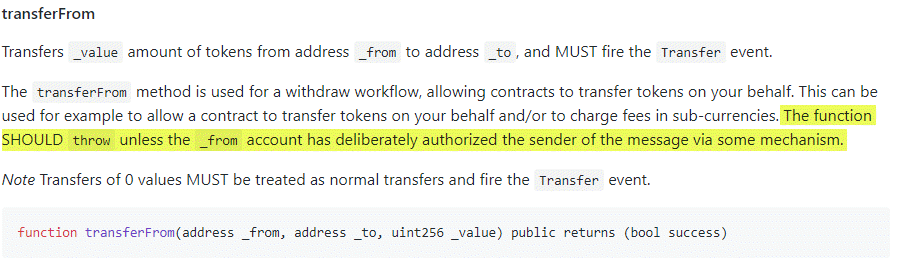
\includegraphics[width=1.0\linewidth]{figures/multiple_withdrawal_30.png}
	\caption{ERC20 \textit{transferFrom} method that emphasizes on throwing exception if spender is not authorized to move tokens.}
\end{figure}

 y this assumption, we secured \textit{transferFrom} method instead of \textit{approve} method by adding required codes to prevent more token transfer that allowed:
 
\begin{figure}[t]
	\centering
	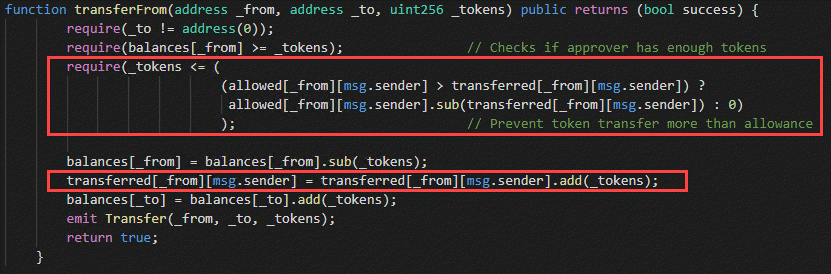
\includegraphics[width=1.0\linewidth]{figures/multiple_withdrawal_31.png}
	\caption{Securing \textit{transferFrom} method instead of \textit{approve} method.}
\end{figure}

In fact, there is no relation between allowance (\textit{allowed[\_from][msg.sender]}) and transferred tokens (\textit{transferred[\_from][msg.sender]}). The fist variable shows maximum transferable tokens by a spender and can be changed irrelative to transferred tokens (i.e., \textit{approve} method does not check transferred tokens). If Bob has not already transferred that much of tokens, he would be able to transfer difference of it \textit{allowed[\_from][msg.sender].sub(transferred[\_from][msg. sender]}). In other words, transferred is life time variable that accumulates transferred tokens regardless of allowance change. This token is implemented as TKNv3\footnote{https://rinkeby.etherscan.io/address/0x5d148c948c01e1a61e280c8b2ac39\newline fd49ee6d9c6} on Rinkby network and passed compatibility by transferring tokens. In terms of gas consumption, \textit{transferFrom} function needs at about 37\% more gas than standard \textit{transferFrom} implementation which is acceptable for having a secure ERC20 token.
